\begin{figure}[ht]
		\centering
		\resizebox{0.75\textwidth}{!}{%
			\begin{tikzpicture}[>=stealth, line width=0.8pt, font=\small,
				nodo/.style  = {circle, fill=white, draw=black,
					inner sep=0pt, minimum size=5pt, line width=0.8pt},
				]
				
				%% ── Parametri geometrici globali ─────────────────────────────────
				\def\L{3.0}      % luce ell
				\def\tw{0.20}    \def\thA{0.34}  \def\thR{0.28}
				\def\sr{0.07}    \def\bw{0.14}   \def\gw{0.26}
				\def\GapP{2.5}   % gap orizzontale tra i due pannelli
				
				%% Posizioni nodi
				\pgfmathsetmacro{\xB}{\L}
				\pgfmathsetmacro{\xG}{0.5*\L}
				\pgfmathsetmacro{\XPb}{\L + \GapP}
				
				%% =================================================================
				%% PANNELLO (a) — PROBLEMA REALE: cedimento in B
				%% =================================================================
				\begin{scope}[xshift=0cm, yshift=0cm]
					
					%% Spostamento verticale del cedimento (unità grafica)
					\def\vb{0.55}
					
					%% Trave indeformata (riferimento, in grigio)
					\draw[line width=0.6pt, gray] (0,0) -- (\xB,0);
					
					%% Trave reale (configurazione deformata, ruotata attorno ad A)
					%% A resta fermo, B scende di vb, G scende di vb/2
					\draw[line width=2.2pt] (0,0) -- (\xB,-\vb);
					
					%% Etichette nodi
					\node[above=0.04] at (0,0)   {$A$};
					\node[above=0.04] at (\xG,0) {$G$};
					\node[above=0.04] at (\xB,0) {$B$};
					
					%% Cerniera in A (resta in posizione)
					\draw (0,0) -- ++(-\tw,-\thA) -- ++(2*\tw,0) -- cycle;
					\draw (-\gw,-\thA) -- (\gw,-\thA);
					\foreach \x in {-0.20,-0.10,0,0.10,0.20}
					\draw[thin] (\x,-\thA) -- ++(-.07,-.09);
					\node[nodo] at (0,0) {};
					
					%% Carrello in B rimosso: indico con pallino bianco la
					%% libertà di traslazione verticale (cedimento imposto)
					\node[nodo] at (\xB,-\vb) {};
					
					%% Cedimento bar v in B: freccia verticale verso il basso
					\draw[->, line width=0.6pt, gray]	(\xB+0.40, 0) -- (\xB+0.40, -\vb);
					\node[font=\footnotesize, right, color=black!60] at (\xB+0.45, -0.5*\vb) {$\bar v$};
					
					
					%% Spostamento eta_G in G: freccia verticale verso il basso, da y=0
					\draw[->, line width=0.6pt, gray] (\xG, 0) -- (\xG, -0.5*\vb);
					\node[font=\footnotesize, right, color=black!60]at (\xG+0.05, -0.27*\vb) {$\eta_G$};
					
					
					%% Etichetta pannello
					\node[font=\small, below=0.05] at (0.5*\xB, -1.10)
					{(a) Problema reale};
					
				\end{scope}
				
				%% =================================================================
				%% PANNELLO (b) — PROBLEMA VIRTUALE: forza unitaria in G
				%% =================================================================
				\begin{scope}[xshift=\XPb cm, yshift=0cm]
					
					%% Trave (struttura integra)
					\draw[line width=2.2pt] (0,0) -- (\xB,0);
					
					%% Etichette nodi
					\node[left=0.04] at (0,0)   {$A$};
					\node[below=0.04] at (\xG,0) {$G$};
					\node[right=0.04] at (\xB,0) {$B$};
					
					%% Cerniera in A
					\draw (0,0) -- ++(-\tw,-\thA) -- ++(2*\tw,0) -- cycle;
					\draw (-\gw,-\thA) -- (\gw,-\thA);
					\foreach \x in {-0.20,-0.10,0,0.10,0.20}
					\draw[thin] (\x,-\thA) -- ++(-.07,-.09);
					\node[nodo] at (0,0) {};
					
					%% Carrello verticale in B
					\draw (\xB,0) -- ++(-\tw,-\thR) -- ++(2*\tw,0) -- cycle;
					\draw (\xB-\gw,-\thR) -- (\xB+\gw,-\thR);
					\draw (\xB-\bw,-\thR-0.10) circle (2pt);
					\draw (\xB+\bw,-\thR-0.10) circle (2pt);
					\draw (\xB-\gw,-\thR-0.20) -- (\xB+\gw,-\thR-0.20);
					\foreach \x in {-0.20,-0.10,0,0.10,0.20}
					\draw[thin] (\xB+\x,-\thR-0.20) -- ++(-.07,-.09);
					\node[nodo] at (\xB,0) {};
					
					%% Forza unitaria 1* in G verso il basso
					\def\Fh{0.85}
					\draw[->, line width=1.0pt] (\xG, \Fh) -- (\xG, 0.05);
					\node[right=0.05, font=\small] at (\xG, 0.5*\Fh) {$1^{*}$};
					
					
					%% Reazioni virtuali R_A^* = 1/2 verso l'alto
					\def\Rh{0.55}
					\draw[->, line width=0.85pt] (0, 0) -- (0, \Rh);
					\node[font=\footnotesize, above]	at (0, \Rh+0.05) {$R_A^{*}=\tfrac{1}{2}$};
					
					%% R_B^* = 1/2 verso l'alto
					\draw[->, line width=0.85pt] (\xB, 0) -- (\xB, \Rh);
					\node[font=\footnotesize, above] at (\xB, \Rh+0.05) {$R_B^{*}=\tfrac{1}{2}$};
					
					
					%% Etichetta pannello
					\node[font=\small, below=0.05] at (0.5*\xB, -1.10)
					{(b) Problema virtuale};
					
					%				\node[font=\small, below=0.05] at (0.5*\xB, -1.55)
					%				{(b) Problema virtuale};
					
				\end{scope}
				
			\end{tikzpicture}%
		}
		\caption{TFV per il calcolo dello spostamento $\eta_G$ in
			una trave semplicemente appoggiata con cedimento in $B$.}
		\label{fig:TFV_cedimento}
	\end{figure}
